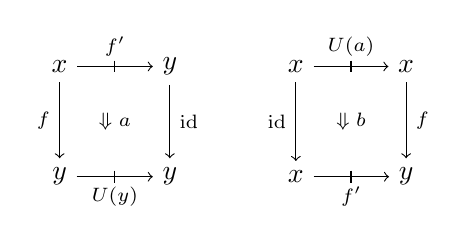
\begin{tikzpicture}
\begin{scope}[shift={(-0.5,0)}]
\node (1) at (-0.2,0.2) {$x$};
\node (2) at (-0.2,-1.2) {$y$};
\node (3) at (1.2,0.2) {$y$};
\node (4) at (1.2,-1.2) {$y$};
\node at (0.5,-0.5) {\scriptsize $\Downarrow a$};
%
\draw [->] (1) edge node [above] {\scriptsize $f'$} (3);
\draw [->] (1) edge node [left] {\scriptsize $f$} (2);
\draw [->] (2) edge node [below] {\scriptsize $U(y)$} (4);
\draw [->] (3) edge node [right] {\scriptsize id} (4);
%
\node (v1) at (0.5,0.4) {};
\node (v2) at (0.5,0) {};
\node (v3) at (0.5,-1) {};
\node (v4) at (0.5,-1.4) {};
%
\draw  (v1) edge (v2);
\draw  (v3) edge (v4);
\end{scope}
%
%
%
\begin{scope}[shift={(2.5,0)}]
\node (1) at (-0.2,0.2) {$x$};
\node (2) at (-0.2,-1.2) {$x$};
\node (3) at (1.2,0.2) {$x$};
\node (4) at (1.2,-1.2) {$y$};
\node at (0.5,-0.5) {\scriptsize $\Downarrow b$};
%
\draw [->] (1) edge node [above] {\scriptsize $U(a)$} (3);
\draw [->] (1) edge node [left] {\scriptsize id} (2);
\draw [->] (2) edge node [below] {\scriptsize $f'$} (4);
\draw [->] (3) edge node [right] {\scriptsize $f$} (4);
%
\node (v1) at (0.5,0.4) {};
\node (v2) at (0.5,0) {};
\node (v3) at (0.5,-1) {};
\node (v4) at (0.5,-1.4) {};
%
\draw  (v1) edge (v2);
\draw  (v3) edge (v4);
\end{scope}
%
%
%
\end{tikzpicture}